% Options for packages loaded elsewhere
\PassOptionsToPackage{unicode}{hyperref}
\PassOptionsToPackage{hyphens}{url}
%
\documentclass[
]{article}
\usepackage{lmodern}
\usepackage{amssymb,amsmath}
\usepackage{ifxetex,ifluatex}
\ifnum 0\ifxetex 1\fi\ifluatex 1\fi=0 % if pdftex
  \usepackage[T1]{fontenc}
  \usepackage[utf8]{inputenc}
  \usepackage{textcomp} % provide euro and other symbols
\else % if luatex or xetex
  \usepackage{unicode-math}
  \defaultfontfeatures{Scale=MatchLowercase}
  \defaultfontfeatures[\rmfamily]{Ligatures=TeX,Scale=1}
\fi
% Use upquote if available, for straight quotes in verbatim environments
\IfFileExists{upquote.sty}{\usepackage{upquote}}{}
\IfFileExists{microtype.sty}{% use microtype if available
  \usepackage[]{microtype}
  \UseMicrotypeSet[protrusion]{basicmath} % disable protrusion for tt fonts
}{}
\makeatletter
\@ifundefined{KOMAClassName}{% if non-KOMA class
  \IfFileExists{parskip.sty}{%
    \usepackage{parskip}
  }{% else
    \setlength{\parindent}{0pt}
    \setlength{\parskip}{6pt plus 2pt minus 1pt}}
}{% if KOMA class
  \KOMAoptions{parskip=half}}
\makeatother
\usepackage{xcolor}
\IfFileExists{xurl.sty}{\usepackage{xurl}}{} % add URL line breaks if available
\IfFileExists{bookmark.sty}{\usepackage{bookmark}}{\usepackage{hyperref}}
\hypersetup{
  pdftitle={Flexible risk-based portfolio optimisation (Github link)},
  hidelinks,
  pdfcreator={LaTeX via pandoc}}
\urlstyle{same} % disable monospaced font for URLs
\usepackage[margin=1in]{geometry}
\usepackage{longtable,booktabs}
% Correct order of tables after \paragraph or \subparagraph
\usepackage{etoolbox}
\makeatletter
\patchcmd\longtable{\par}{\if@noskipsec\mbox{}\fi\par}{}{}
\makeatother
% Allow footnotes in longtable head/foot
\IfFileExists{footnotehyper.sty}{\usepackage{footnotehyper}}{\usepackage{footnote}}
\makesavenoteenv{longtable}
\usepackage{graphicx,grffile}
\makeatletter
\def\maxwidth{\ifdim\Gin@nat@width>\linewidth\linewidth\else\Gin@nat@width\fi}
\def\maxheight{\ifdim\Gin@nat@height>\textheight\textheight\else\Gin@nat@height\fi}
\makeatother
% Scale images if necessary, so that they will not overflow the page
% margins by default, and it is still possible to overwrite the defaults
% using explicit options in \includegraphics[width, height, ...]{}
\setkeys{Gin}{width=\maxwidth,height=\maxheight,keepaspectratio}
% Set default figure placement to htbp
\makeatletter
\def\fps@figure{htbp}
\makeatother
\setlength{\emergencystretch}{3em} % prevent overfull lines
\providecommand{\tightlist}{%
  \setlength{\itemsep}{0pt}\setlength{\parskip}{0pt}}
\setcounter{secnumdepth}{5}
\usepackage[]{natbib}
\bibliographystyle{plainnat}

\title{Flexible risk-based portfolio optimisation
\href{https://github.com/jhlandman/flex_rb_opt}{\emph{(Github link)}}}
\author{Emlyn Flint\footnote{Legae Peresec}, Jayson Landman\footnote{Ninety One Asset Management}}
\date{2020-07-05}

\begin{document}
\maketitle
\begin{abstract}
The purpose of this study is to present and test a general framework for risk-based investing. It permits various risk-based portfolios such as the global minimum variance, equal risk contribution and equal weight portfolios. The framework also allows for different estimation techniques to be used in finding the portfolios. The design of the study is to collate the existing research on risk-based investing, to analyse some modern methods to reduce estimation risk, to incorporate them in a single coherent framework, and to test the result with South African equity data. The techniques to reduce estimation risk draw from the usual mean-variance and risk-based optimisation literature. The techniques include regime switching, quantile regression, regularisation and subset resampling. In the South African experiment, risk-based portfolios materially outperformed the market weight portfolio out-of-sample using a Sharpe ratio measure. Additionally, the global minimum variance portfolio performed better than other risk-based portfolios. Given the long estimation window, no estimation techniques consistently outperformed the application of sample estimators only.

\textbf{Keywords}: risk-based investing, portfolio optimisaiton, estimation risk.
\end{abstract}

{
\setcounter{tocdepth}{2}
\tableofcontents
}
\hypertarget{about}{%
\section{About}\label{about}}

This is a research paper created with the \texttt{bookdown} package in R. It is intended to promote
reproducibility in academic research.

\hypertarget{introduction}{%
\section{Introduction}\label{introduction}}

If a risk-averse investor wants to construct portfolios with desirable properties, they would
ideally want to find allocations that offer an attractive risk-reward trade-off. \citet{M52} developed
modern portfolio theory and introduced the mean-variance optimal portfolio as a quantitative
solution to this asset allocation problem. However, the reward derived from this portfolio has to be
estimated from sample data and is often difficult to accurately predict - which, in turn, leads to
Markowitz's mean-variance portfolio being highly sensitive to the estimated portfolio inputs.

As an alternative, risk-based investing provides an avenue for finding portfolios for which expected
returns do not need to be estimated, and therefore resolves the portfolio expected return
sensitivity problem. Examples of risk-based portfolios commonly seen in practice are the global
minimum variance portfolio, the equal risk contribution portfolio, and the equal weight portfolio.
These three portfolios are optimal for investors that prioritise weight diversification, risk
diversification, or a specific combination of both.

Nevertheless, risk-based portfolios remain sensitive to covariance matrix estimation and hence
estimation risk. Improving risk-based estimation is done in three ways in this research. The first
improvement alters the covariance estimation procedure by accounting for differences in the sample
data. These changes include grouping to account for both non-normality and state-based
inhomogeneity. The second involves penalising the optimisation to limit the range of admissable
portfolios, which increases the investor's odds of choosing a well-estimated portfolio. The final
enhancement changes the implementation methodology entirely by performing the portfolio optimisation
on subsets of assets and then resampling to find an aggregate portfolio.

This research aims to bring together useful elements of risk-based portfolio estimation and
construction methodology into a single flexible framework. The general structure allows a choice of
risk-based portfolio as well as estimation risk reduction technique to improve the out-of-sample
portfolio performance. Once we have established a framework, the specific portfolio and estimation
technique, examples are developed theoretically. All of these reforms will be hollow without being
applied to actual financial data. Therefore, the various estimation techniques and risk-based
portfolio pairs are back-tested using South African equity data in an experiment, with the results
being measured by standard performance methodologies.

This research is built on the work of several different authors. Firstly - as with nearly all
portfolio construction research - this dissertation hinges on the modern portfolio theory of \citet{M52}.
It then considers the particular case of risk-based investing and makes use of the generalised
frameworks introduced by \citet{J13} and \citet{RR15}. Finally, in terms of improving the estimation and
optimisation processes, we make use of the ideas investigated by \citet{FD18}, \citet{K18}, and \citet{SW17}.

The rest of this dissertation is set out as follows. Chapter 2 outlines a general framework for
constructing risk-based portfolios and estimating them in a robust manner. Chapter 3 gives an
overview of the specific risk-based portfolios considered in this work. Chapter 4 presents several
techniques for reducing estimation risk, exploring their theoretical underpinnings and providing
general intuition. Chapter 5 then considers the empirical application of these techniques,
highlighting several technicalities. Chapter 6 then applies the flexible risk-based framework to SA
equity data, providing an empirical comparison of different implementations. Chapter 7 concludes the
research and provides avenues for further research.

\hypertarget{genframework}{%
\section{A framework for constructing risk-based portfolios}\label{genframework}}

\hypertarget{mpt}{%
\subsection{An overview of modern portfolio theory}\label{mpt}}

Every investor has a universe of \(N\) assets to which they can allocate capital. The proportion of
their allocation to the \emph{i}\(^{\text{th}}\) asset, \(w_i\), depends on the investor's risk and return
preferences. They could prefer riskier asset combinations because they require high capital growth,
or they could prefer more stable asset combinations that prioritise capital preservation. The column
vector \(w = [w_1,w_2,\text{…},w_N]^\intercal\) is an \(N \times 1\) vector of allocations that define an
investor's portfolio. This portfolio is constrained by the investor's capital budget, which may be
articulated through the notion of weights. Therefore, all considered portfolios should adhere to the
budget constraint: \(\sum_i w_i = 1\).

In his seminal paper, \citet{M52} attempts to quantify the asset allocation process. Herein he posits that
the investor has to make a risk-reward trade-off when considering their portfolio returns,
\(R_\mathrm{p}\), over a pre-determined time horizon \([0, T]\). In his framework, he measures risk with
the variance of portfolio returns \(\mathbb{V}\mathrm{ar}[R_\mathrm{p}] = w^\intercal \Sigma w\),
where \(\Sigma\) is the \(N \times N\) asset return covariance matrix. Markowitz measures reward by the
expectation of portfolio returns \(\mathbb{E}[R_\mathrm{p}] = w^\intercal \mu\), where \(\mu\) is the
\(N \times 1\) vector of expected asset returns. If the investor fixes expected returns to a constant,
\(\mathbb{E}[R_\mathrm{p}] = c\), they encounter the problem of minimising portfolio risk,
\(\mathbb{V}\mathrm{ar}[R_\mathrm{p}]\). The mean-variance optimal (MVO) portfolio \(w_\mathrm{mvo}\)
achieves this goal while adhering to the budget constraint and the fixed expected return constraint.
Written mathematically, \(w_\mathrm{mvo}\) is the solution to the following Markowitz optimisation:
\begin{align} 
w_\mathrm{mvo} &= \underset{w}{\text{argmin}} \Big \{ w^\intercal \Sigma w \Big \},
\label{eq:mvoone}
\end{align}
subject to the constraints:
\begin{align*}
\mathcal{C}(w) &= 
\begin{cases}
 w^\intercal \mu &= c \;\;\;  \\
w^\intercal \underline{1} &= 1 \;\; .
\end{cases}
\end{align*}

There is a complication when using this framework in practice because \(\Sigma\) and \(\mu\) are
unknown. The investor can only observe a small set of sample returns from the underlying stock
processes that use these quantities as inputs. The sample returns, represented by a \(N \times T\)
matrix \(\textbf{X}\), can be used to estimate \(\Sigma\) and \(\mu\). The sample estimates are:

\begin{align}
\textbf{S}&=  \frac{1}{T - 1}(\textbf{X} - \mathbf{\bar{x}} \underline{1}^\intercal_T)(\textbf{X} - \mathbf{\bar{x}} \underline{1}^\intercal_T)^\intercal, \label{eq:samplevar} \\
\mathbf{\hat{\mu}} &= \mathbf{\bar{x}} , \label{eq:samplemean}
\end{align}
where \(\mathbf{\bar{x}}\) is a \(N \times 1\) vector of mean returns. A total of \(\frac{N(N+1)}{2}\)
distinct parameters are being estimated for the sample covariance matrix (SCM) while \(N\) distinct
sample expected returns are estimated. \(\textbf{S}\) and \(\hat{\mu}\) can be substituted into
equation \eqref{eq:mvoone} to infer an MVO portfolio, \(\hat{w}_\mathrm{mvo}\). For each level of
portfolio return \(c = \hat{w}^\intercal \hat{\mu}\), an estimated portfolio volatility level
\(\mathbb{SD}[\hat{R}_\mathrm{p}] = \sqrt{\hat{w}^\intercal\textbf{S}\hat{w}}\) is realised. These
estimated expected return-volatility pairs induce a frontier in the expected return-volatility
plane, which may or may not be close to the frontier implied by the actual inputs \(\Sigma\) and
\(\mu\). The actual frontier is optimal for the Markowitz framework, and he terms it the `efficient
frontier'.

The above framework and estimation procedure yields a solution to the asset allocation dilemma, but
there is still a sensitivity predicament. \citet{M89} shows that the MVO procedure, as described above,
overweights assets with substantial estimated returns \(\mathbf{\bar{x}}\). However, these are the
same assets that are likely to have been misestimated. Thus, any potential estimation errors are
`maximised' - an undesirable property that makes \(\hat{w}_\mathrm{mvo}\) a potential liability for
the investor to hold.

The MVO procedure is commonly adjusted to reduce sensitivity to the input \(\mathbf{\bar{x}}\) in one
of two ways. The first is to estimate expected returns in a manner that targets return drivers or
factors, which has motivated the rise of factor-based investing \citep{A14}. The second adjustment is to
remove the dependency on expected return estimates altogether and only construct portfolios based
on their risk properties. The latter has inspired the field of risk-based investing and is the
focus of this dissertation.

\hypertarget{introducing-risk-based-investing}{%
\subsection{Introducing risk-based investing}\label{introducing-risk-based-investing}}

A general risk-based portfolio optimisation programme is given below in equation \eqref{eq:rbintro}.
Removing the expected return constraint and altering the previous MVO optimisation problem for the
consideration of a generalised objective risk function \(f(\cdot| \textbf{X})\) yields:
\begin{align}
w^* = \underset{w}{\text{argmin}} \Big \{ f(w, \Sigma| \textbf{X}) \Big \}, \label{eq:rbintro}
\end{align}
subject to the constraint:
\begin{align*}
w^\intercal \underline{1} &= 1 \;\; ,
\end{align*}

where \(f(\cdot | \textbf{X})\) is a risk metric to be minimised. The choice of \(f(\cdot | \textbf{X})\) determines which risk-based portfolio is the optimal solution. Chapter \textbf{make
chapeter} expounds on the risk-based portfolio types relevant to this research.

The range of feasible portfolios given by equation \eqref{eq:rbintro} is practically too general
because unlikely single asset weights are still possible. To this end, an investor should apply a
weight constraint to limit feasible allocations, ensuring comparability with practical investing.
\citet{JM03} show that risk-based long-short portfolios can have extreme weights in practice, which are
unlikely to be accepted by an investor.

Additionally, \citet{JM03} also conclude that imposing the long-only investment constraint on US equities
leads to improved efficiency for optimal portfolios constructed with the first two sample moments
\(\hat{\mu}\) and \(\textbf{S}\). Hence, applying the long-only constraint is both statistically
appropriate and practically relevant for most investors.

Equally important is that an investor will be reluctant to concentrate their portfolio in a small
number of assets. Limiting the maximum single asset allocation to a selected weight \(\alpha\) avoids
such concentration. These constraints are concurrently expressed as
\(\{w :0 \leq w_i \leq \alpha, \; \forall i \}\) and can be added to optimisation \eqref{eq:rbintro}.
In its current form, the developed framework is still somewhat abstract, so it is not obvious how
to improve it. Even so, one can always define specific properties that the framework ought to have
for there to be a good chance of it operating as intended.

\hypertarget{improving-risk-based-portfolios}{%
\subsection{Improving risk-based portfolios}\label{improving-risk-based-portfolios}}

\citet{H23} defines a mathematical problem as `well-posed' if:

\begin{enumerate}
\def\labelenumi{\arabic{enumi}.}
\tightlist
\item
  the solution exists,
\item
  the solution is unique,
\item
  the solution is not overly sensitive to small perturbations in inputs.
\end{enumerate}

Well-posed problems are easier to work with and are more stable than ill-posed problems - ones that
fall short of the definition. The expected return constraint was previously disregarded for MVO
portfolios because the MVO framework often does not meet requirement 3. when the sample mean returns
estimate \(\mu\). Risk-based portfolios are therefore more `well-posed' than MVO portfolios.

However, there are two common ways in which risk-based portfolios are also ill-posed. The first is if
there are very few sample observations; namely, if \(T < N\). In this scenario, the covariance matrix
is not of full rank and is therefore not invertible, causing non-unique solutions to \(w^*\). The
framework is then ill-posed by 2. The second is if small changes in \(\textbf{X}\) result in large
deviations of \(w^*\). The framework is then ill-posed by 3. Many researchers such as \citet{JK81}
and \citet{B91} have shown that the latter phenomenon is observed in practice, and often persists even
if \(T\) is much larger than \(N\). To address point (iii) and make the problem well-posed, one needs a
measure of sensitivity. We outline a pseudo-derivation of a sensitivity measure below.

\citet{K18} views the portfolio optimisation problem from a modelling perspective. The returns on the
portfolio are modelled directly by an unknown function \(g(\cdot)\):
\begin{align}
R_p & = g(\textbf{X}) + \epsilon, \label{eq:retmodel}
\end{align}
where \(\epsilon\) has the normal distribution with zero mean and variance \(\phi^2\). Estimating
\(g(\cdot)\) is the aim of using the framework, and it is a real-valued function that is not
necessarily differentiable or continuous. Each algorithm \(q\) refers to a combination of estimation
procedure for the inputs, and a computation of a risk-based portfolio using equation
\eqref{eq:retmodel}. Each \(q\) specifies an estimate of the function \(g\), denoted \(\hat{g}_q\). In the
same way that \(\hat{w}^*\) (\(w^*\) calculated with sample inputs \(\textbf{S}\) and \(\hat{\mu}\)) can be
used to estimate the out-of-sample risk-based portfolio, \(\hat{g}_q\) can predict out-of-sample
portfolio returns, which are forecasted most accurately by the unobservable function \(g\).

It is necessary to distinguish between the two types of data that are available. The first is
historical data comprising of the matrix \(\textbf{X}_0\) and in-sample returns \(R_{\mathrm{p}, 0}\),
which combine to form the set \(\mathcal{H}_0\). The second is out-of-sample data \(\textbf{X}_1\) and
\(R_\mathrm{p, 1}\), which combine to form the set \(\mathcal{H}_1\). Algorithm \(q\) does not utilise the
data contained in \(\mathcal{H}_1\), which are chronologically realised after the most recent points in
\(\mathcal{H}_0\). A mean squared error penalty is appropriate to measure the accuracy with which
\(\hat{g}_q (\textbf{X}_1)\) (estimated using \(\mathcal{H}_0\)) predicts the out of sample returns
\(R_\mathrm{p, 1}\). \citet{K18} terms the expectation of the out-of-sample mean squared error
``generalisation error'' (GE), shown mathematically as:
\begin{align}
GE(\hat{g}_q) & = \mathbb{E}[(R_\mathrm{p, 1} - \hat{g}_q (\textbf{X}_1))^2|{\mathcal{H}_1}],
\end{align}
where GE is specific to a sample. The actual quantity of interest is the expected performance of \(q\)
for many potential sample sets, as we are evaluating \(q\)'s efficacy holistically. This quantity is
called the expected generalisation error across all samples, denoted \(G_q\). Furthermore, \(G_q\) may be
decomposed \footnote{The decomposition is shown by \citet{FHT01}.} to reflect a common modelling trade-off between
bias and variance:
\begin{align}
G_q &:= \mathbb{E} \Big [ \mathbb{E}[(R_\mathrm{p, 1} - \hat{g}_q (\textbf{X}_1))^2|{\mathcal{H}_1}] \Big | \mathcal{H}_0\Big ] , \\
& = \underbrace{ \Big (g(\textbf{X}_1) - \mathbb{E}[\hat{g}_q (\textbf{X}_1)|\mathcal{H}_0] \Big )^2}_{\text{squared bias}} + \underbrace{\mathbb{V}\mathrm{ar} [\hat{g}_q(\textbf{X}_1)|\mathcal{H}_0]}_{\text{variance}} + \underbrace{\phi^2}_{\text{irreducible error}}.\label{eq:bvdecomp}
\end{align}
The squared bias is the extent to which the expectation of predicted returns differs from the best
possible predictor of returns, the correct function \(g(\cdot)\). The variance measures the magnitude
by which the predicted returns will vary under repeated sampling. By setting
\(\hat{g}_q(\cdot) = g(\cdot)\) in equation \eqref{eq:bvdecomp} only statistical noise remains; hence,
the noise is irreducible. The risk of misestimating \(g(\cdot)\) should not include the risk that is
retained by even the best estimator. Therefore, estimation risk is considered as the sum of the first
two terms only, the squared bias and the variance. An over-fitted algorithm will have high variation
for repeated samples. An under-fitted algorithm will have high bias and be consistently poor for
repeated samples. The over- and under-fitting trade-off is an example of how the bias-variance
trade-off works in practice.

Until now, we have assumed that the estimated portfolio \(\hat{w}^*\) from equation \eqref{eq:rbintro}
is an unbiased estimate of the actual risk metric-minimising portfolio \(w^*\) because the choice of
\(f(\cdot | \textbf{X})\) determines precisely the type of risk-based portfolio. However,
\(f(\cdot|\textbf{X})\) does not precisely determine the estimation risk. Employing a penalty on the
objective function introduces bias to reduce estimation risk, \emph{i.e.} hopefully, the squared
bias increase does not outweigh the variance decrease. The introduction of the penalty yields an
estimated portfolio \(\hat{w}^*\) that is consistently closer to \(w^*\) than an unbiased portfolio would
be. The penalty constraint can be stated as \(P(w) \leq s\) and reduces the set of all possible
portfolios. If done correctly allocations that are misestimated by the heftiest margins are excluded
by this constraint, and allocations that are consistently closer to the actual portfolio remain. The
general risk-based framework can now be restated as below to accommodate the penalty using a
Lagrangian multiplier approach:
\begin{align}
w^* = \underset{w}{\text{argmin}} \Big \{ f(w, \Sigma| \textbf{X}) + \lambda P(w) \Big \}, \label{eq:genopt}
\end{align}
subject to the constraints:
\begin{align*}
\mathcal{C}(w) &= 
\begin{cases}
w^\intercal \underline{1} = 1 \;\; \\
0 \leq w_i \leq \alpha, \; \forall i \;\;\; ,
\end{cases}
\end{align*}

where \(P(\cdot)\) is the penalty function, and \(\lambda\) is the Lagrangian multiplier. Kinn proposes
estimating \(\lambda\) in a way that is consistent with the rest of the optimisation. Therefore, we
apply the \(\lambda\) estimation that minimises the portfolio specific risk metric using in-sample
data. Additionally, by setting \(\lambda = 0\), the unpenalised portfolio can still be recovered.
Optimisation \eqref{eq:genopt} will be the general risk-based portfolio optimisation going forward.

Improving on the vanilla risk-based optimisation is done in three ways in this research, and these
improvements are also common in the literature. Approach one deals with the assumption in equation
\eqref{eq:retmodel} that \(\epsilon\) has a normal distribution, and that the errors through time are
independent and identically distributed. If \(\hat{g}_q\) fails to approximate \(g\) correctly, then the
assumption is violated. There could be natural heterogeneity in the data accounted for by \(g\). \citet{FD18}
attempt to deal with heterogeneity by changing the estimation procedure of \({g}\) so that it includes
and accounts for potential differences in each observation of sample data. They do this through the
application of regimes and quantiles, grouping the input data to increase the accuracy of the
estimated model. The second approach adapted from \citet{K18} has already been shown above and
involves penalising the optimisation and setting \(\lambda > 0\) in equation \eqref{eq:genopt}. The
third and final approach requires resampling from the observations in \(\textbf{X}\) for different
subsets of assets and hinges on implementation adjustments. \citet{SW17} suggest finding \(w^*\)
multiple times for different resampled subsets and blending the result afterwards to find an
aggregate weight, that hopefully reduces estimation risk. Chapter \textbf{insert chapter ref} contains a
more detailed exploration of these techniques. Before that, further investigation of desirable risk
properties and the portfolios that have them is required to specify \(f(\cdot|\textbf{X})\).

\hypertarget{rbportch}{%
\section{Overview of risk-based portfolios}\label{rbportch}}

There are many types of risk-based portfolios, for a broader analysis refer to \citet{DV17}. In this chapter,
we review three risk-based portfolios: the global minimum variance, equal weight and equal risk
contribution portfolios. The risk properties that these portfolios have, the strategies that bear them
out and the conditions under which they perform optimally are all covered.

\hypertarget{risk-based-portfolio-types}{%
\subsection{Risk-based portfolio types}\label{risk-based-portfolio-types}}

Each risk-based portfolio is optimal in some sense because they all minimise a specific objective risk
function. The nature of the objective function depends on the investor's risk preferences. In line
with \citet{M52}, a genetic risk metric to minimise is the portfolio variance, as an investor may not be
willing to tolerate large swings in capital value. Setting
\(f(\cdot|\textbf{X}) = w^\intercal \Sigma w\) in portfolio optimisation \eqref{eq:genopt} yields the
global minimum variance (GMV) portfolio, denoted \(w_\textrm{gmv}\). The objective function is the same
as for the MVO portfolio for an imputed value of \(c\), meaning that the GMV portfolio sits on the
efficient frontier. The GMV portfolio is also the only risk-based portfolio that is always on the
efficient frontier.

\citet{MRT10} utilise the concept of an asset's marginal risk contribution (MRC) in a portfolio to perform
risk-based portfolio calculations. It is the sensitivity of the portfolio volatility to the weight of
an asset in a portfolio. Alternative representations of the MRC and an outline of why the weighted sum
of the MRC's is minimised for the GMV portfolio are shown in appendix \textbf{insert appendix ref}. Below
is the mathematical definition of the MRC for the \(i^{\mathrm{th}}\) asset:
\begin{align}
\frac{\partial}{\partial w_i} \Big [ \sigma(w) \Big ]= \frac{(\Sigma w)_i}{\sqrt{w^\intercal \Sigma w}}.
\end{align}

When taking the realised portfolio returns as the single risk factor, there is no idiosyncratic risk
present for assets in the portfolio against this factor. Accordingly, the GMV portfolio is the lowest
possible beta portfolio. The GMV portfolio is, therefore, optimal for the investor that always takes
on the least risk at the margin. However, risk has to be estimated, so the investor only knows what
the least risky options available to them are in a historical sense. The downside is that always
choosing the lowest marginal risk contributing asset is implicitly displaying a high level of
confidence in estimations of risk.

Contrastingly, the investor may be at a loss when estimating risk. The only measure of diversification
for such an investor is weight diversification. To minimise their risk taken at the margin, this
investor would hold the smallest possible weight in each of the assets while still satisfying the
constraints. This strategy ensures that the investor avoids the maximum marginal risk contributing
asset to the greatest extent possible given that they are unsure which of the \(N\) assets it is. The
least weight concentrated portfolio that this strategy alludes to is the equal weight (EW) portfolio:

\begin{align}
w_{ew} & = \Big [\frac{1}{N} \; \cdot \cdot \cdot \frac{1}{N} \Big ]^\intercal \; ,
\end{align}

where the weight diversification measure that this portfolio maximises is the inverse Herfindahl index
(IHI), calculated as \(H^{-1} (w) = (\sum_{i = 1}^N w_i^2)^{-1}\). The most weight concentrated
portfolio is the single asset portfolio - where a single non-zero asset weight is \(1\). The IHI of this
portfolio is \(1\), which is as low as it can be. On the other hand, the EW portfolio has an IHI value
of \(N\). All portfolios, therefore, have an IHI on the interval \([1, N]\). In the presence of a maximum
weight constraint, the lower bound of the interval changes. The new lower bound is derived in appendix
\textbf{insert appendix ref}. To find the EW portfolio using framework \eqref{eq:genopt}, set the objective
function to the Herfindahl index, \(f(\cdot|\textbf{X}) = \sum_{i = 1}^N w_i^2\). No parameters in the
objective function require estimation, so this is a sample return independent optimisation, which
reflects the investor's lack of confidence in historical data.

The GMV and EW portfolios represent two extremes of investors, specifically those that value
volatility reduction only and those that value weight diversification only. The inequality
\(\sigma(w_{gmv}) \leq \sigma(w^\diamond) \leq \sigma(w_{ew})\) verifies this intuition. The portfolio
\(w^\diamond\) has intermediate weight concentration. Proof of the inequality is given in appendix
\textbf{insert appendix ref}. It is unlikely that a capital allocator will completely disregard one
risk-based approach for another. One method to construct a sound intermediate portfolio that
incorporates the MRC philosophy from the GMV portfolio construction and the high risk-asset avoidance
philosophy from the EW portfolio construction is to equalise the total risk contribution (TRC) from
each asset. An asset's TRC is the product of its MRC and its weight in the portfolio:
\begin{align*}
\text{TRC}_i &= w_i \cdot \frac{\partial}{\partial w_i} \Big [ \sigma(w)\Big ], \\
& = \frac{w_i \cdot (\Sigma w)_i}{\sqrt{w^\intercal \Sigma w}},
\end{align*}
where TRC's sum to the portfolio volatility. An equal risk contribution (ERC) portfolio equalises all
of the TRC's so that no single asset is a comparatively significant contributor to risk. The choice of
\(f(\cdot|\textbf{X})\) that minimises the squared distances between the TRC's to the greatest extent
possible is given below:
\begin{align}
f(w, \Sigma|\textbf{X}) &= \sum_{i = 1}^N  \sum_{j \geq i}^N(w_i(\Sigma w)_i - w_j(\Sigma w)_j)^2 \;\;  .
\end{align}

\citet{MRT10} show that a log-constraint on the weights in GMV optimisation could equivalently express this
choice of \(f(\cdot| \textbf{X})\) - an idea explored further in appendix \textbf{insert appendix ref}.
Therein it is shown that the ERC portfolio is an intermediate portfolio \(w^\diamond\). While there are
several other risk-based portfolios that have been suggested in the literature, we will focus our
attention only on these three portfolios, which are arguably some of the most common risk-based
portfolios seen in practice \citet{J13}.

\hypertarget{risk-based-portfolio-properties}{%
\subsection{Risk-based portfolio properties}\label{risk-based-portfolio-properties}}

Section \ref{mpt} introduces the Markowitz efficient frontier. \citet{S64} extends this work to deduce that
there is an optimal portfolio called the tangency portfolio. He does make certain assumptions about
investors' preferences and the presence of a risk-free asset. The market-weighted (MW) portfolio is the
portfolio for which the efficient frontier is tangential to the line bisecting the y-axis at the
risk-free rate (\(r_\mathrm{f}\)) in the expected return-volatility plane. The MW portfolio is the
portfolio held by all investors in the market on average and is relevant because it offers the investor
diversification with negligible transaction costs \citet{P07}. The MW portfolio is not risk-based in the
traditional sense, but it does not require an estimate of expected returns to calculate; hence, the MW
portfolio offers a cheap benchmark against which to compare risk-based portfolio performance. However,
the holder of the MW does implicitly adopt all investors' weighted expectations of expected returns
\citet{H91}. The tangency portfolio is optimal for the Sharpe ratio (SR) measure under Sharpe's
assumptions. The measure is defined as:
\begin{align}
\text{SR}_\mathrm{p} = \frac{\mathbb{E}[R_\mathrm{p}] - r_\mathrm{f}}{\mathbb{SD}[R_\mathrm{p}]} \;.
\end{align}

Within the MVO construction, the MW portfolio has the maximum Sharpe ratio (MSR) and is, therefore, the
MSR portfolio. \citet{S07} shows that the MSR portfolio, \(w_\mathrm{msr}\), can alternatively be expressed
as the portfolio for which marginal excess returns and the MRC's are equal for all portfolio
constituents. \citet{J13} use this fact to find MSR optimality conditions for each of the risk-based
portfolios, some examples of which are shown in appendix \textbf{insert appendix num}.

Table \ref{tab:rbportprops} summarises the salient risk properties of the EW, ERC, and GMV
portfolios. Included is the strategy to find the portfolio, the requirements for when the portfolio
coincides with the MSR portfolio, and their empirical risk characteristics. The risk characteristics
entail whether the risk is inherent to the investment, the construction of the portfolio, or liquidity
restrictions when creating the portfolio.

\begin{longtable}[]{@{}llll@{}}
\caption{\label{tab:rbportprops} Risk-based investing portfolio properties \citet{J13}}\tabularnewline
\toprule
\begin{minipage}[b]{0.06\columnwidth}\raggedright
Portfolio\strut
\end{minipage} & \begin{minipage}[b]{0.09\columnwidth}\raggedright
Strategy\strut
\end{minipage} & \begin{minipage}[b]{0.39\columnwidth}\raggedright
MSR conditions\strut
\end{minipage} & \begin{minipage}[b]{0.34\columnwidth}\raggedright
Risk characteristics\strut
\end{minipage}\tabularnewline
\midrule
\endfirsthead
\toprule
\begin{minipage}[b]{0.06\columnwidth}\raggedright
Portfolio\strut
\end{minipage} & \begin{minipage}[b]{0.09\columnwidth}\raggedright
Strategy\strut
\end{minipage} & \begin{minipage}[b]{0.39\columnwidth}\raggedright
MSR conditions\strut
\end{minipage} & \begin{minipage}[b]{0.34\columnwidth}\raggedright
Risk characteristics\strut
\end{minipage}\tabularnewline
\midrule
\endhead
\begin{minipage}[t]{0.06\columnwidth}\raggedright
EW\strut
\end{minipage} & \begin{minipage}[t]{0.09\columnwidth}\raggedright
Equalise \(w_i\)\strut
\end{minipage} & \begin{minipage}[t]{0.39\columnwidth}\raggedright
Identical excess returns. Identical volatilities. Identical correlations.\strut
\end{minipage} & \begin{minipage}[t]{0.34\columnwidth}\raggedright
Medium to high risk. Insensitive to \(\Sigma\). Low turnover.\strut
\end{minipage}\tabularnewline
\begin{minipage}[t]{0.06\columnwidth}\raggedright
ERC\strut
\end{minipage} & \begin{minipage}[t]{0.09\columnwidth}\raggedright
Equalise \(TRC_i\)\strut
\end{minipage} & \begin{minipage}[t]{0.39\columnwidth}\raggedright
Identical Sharpe ratios. Identical correlations.\strut
\end{minipage} & \begin{minipage}[t]{0.34\columnwidth}\raggedright
Medium risk. Moderately sensitive to \(\Sigma\). Medium turnover.\strut
\end{minipage}\tabularnewline
\begin{minipage}[t]{0.06\columnwidth}\raggedright
GMV\strut
\end{minipage} & \begin{minipage}[t]{0.09\columnwidth}\raggedright
Equalise \(MRC_i\)\strut
\end{minipage} & \begin{minipage}[t]{0.39\columnwidth}\raggedright
Identical excess returns.\strut
\end{minipage} & \begin{minipage}[t]{0.34\columnwidth}\raggedright
Lowest risk. Highly sensitive to \(\Sigma\). High turnover.\strut
\end{minipage}\tabularnewline
\bottomrule
\end{longtable}

While the MSR conditions are theoretically compelling, out-of-sample optimality is harder to determine
in practice. \citet{H91} show that portfolios that are superior to the MW portfolio exist when:
short-selling is restricted, investments are taxed, and foreign investors are active market
participants. These portfolios should have the same expected return as the MW portfolio with lower
volatility. Their statement is true even in an `efficient market'. Studies of the historical
performance show that some portfolios outperform others. In these studies, the authors restrict the
asset universe to US equities; hence, their results will not necessarily translate to South Africa.
The hope of introducing risk-based portfolios is to find Haugen and Baker's superior portfolios.
Evidence supporting this ambition exists. \citet{DGL07} demonstrate the robust out-of-sample
performance of EW portfolios when compared to MVO and MW portfolios for a broad range of asset
universes. \citet{C06} also demonstrate that GMV portfolios show outperformance against the MW and MVO
benchmarks. They initially attribute this to the diachronic persistence of covariances when compared
to expected returns. In a later paper, \citet{C11} suggest that the outperformance is due to a bias
inherent in the portfolio construction towards stocks that do not move with the rest of the market,
but that still have comparatively high expected returns.

Within risk-based portfolios, \citet{K10} have shown that GMV portfolios outperform EW portfolios when the
implementer uses a long enough estimation window. Therefore, they establish a defence for using
optimisation on a sample covariance matrix. This research remains consistent with these findings,
using the EW portfolio as a benchmark in pursuit of better out-of-sample performance within the GMV
and ERC frameworks. In the next chapter, we outline the techniques used to achieve this aim.

\hypertarget{estriskreduce}{%
\section{Estimation risk reduction techniques}\label{estriskreduce}}

As stated in chapter \ref{genframework}, estimation risk is comprised of squared bias and variance.
There are many methods to approach reducing estimation risk, but in this research, we introduce three
ways that are consistent with the general risk-based investing framework presented in equation
\eqref{eq:genopt}. The first method deals with improving the estimation of the inputs to the risk-based
portfolio function \(f(w, \Sigma|\textbf{X})\), accounting for heterogeneity in the input data. The
second method involves penalising the optimisation objective function to obtain a portfolio estimate
with consistently lower deviation from the actual out-of-sample risk-based portfolio solution. The
final process entails changing the implementation method in a manner that reduces estimation risk.
Every risk reduction technique falls into one of these three categories.

\hypertarget{improving-optimisation-inputs}{%
\subsection{Improving optimisation inputs}\label{improving-optimisation-inputs}}

The first approach to improving on the sample ERC and GMV portfolios involves finding better estimates
for the input \(\Sigma\), given the set of sample returns. As stated in equation \eqref{eq:retmodel},
the function \(g\) deals with the sample returns in a manner that ensures the irreducible error,
\(\phi^2\), is independent and identically normally distributed. However, because \(g\) is unobservable,
our estimation \(\hat{g}\) might not ensure this property. Heterogeneity of sample errors for investment
portfolios has been observed in empirical finance by \citet{AC02}, who demonstrate that negative stock
price correlations are less pronounced in downward markets. Therefore, empirical finance suggests two
states of the world, one where the market is in turmoil, and one where the market is not.

\citet{K12} use these two states to determine separate multi-asset allocations for `turbulent' and `quiet'
markets and adopt a regime switching (RS) approach. To define two regimes, a metric to measure
turbulence is required. The authors take a squared Mahalanobis distance (SMD) approach to determine an
index through time. The Mahalanobis distance is a multi-dimensional generalisation of the notion of how
many standard deviations a point is away from the mean of a distribution. The SMD index (\(d_t\)) is
expressed mathematically as:
\begin{align}
d_t = (R_t - \mu)\Sigma^{-1}(R_t - \mu)^\intercal,
\end{align}
where: \[d_t = \mu_{s_t} + \sigma_{s_t}\epsilon_t,\] and \(\epsilon_t\) has a standard normal
distribution. The state at time \(t\) is shown by the random variable \(s_t\). As asserted earlier, the two
states are Quiet (\(Q\)) and Turbulent (\(T\)), hence \(s_t \in \{Q, T\}\). To calculate the SMD, we require
the unobservable inputs \(\Sigma\) and \(\mu\). They can be replaced by their sample counterparts,
\(\textbf{S}\) and \(\hat{\mu}\), to yield \(\hat{d}_t\). The SMD has a state-specific mean and volatility;
hence different values are observed based on the current system state. If the system emits large values
of \(\hat{d}_t\), the probability of being in a turbulent market is high. If the system emits small
values of \(\hat{d}_t\), the likelihood of being in a quiet market is high. The \(\zeta^{th}\) quantile of
the sample SMDs is the point where the system of reference changes. The market state is also an
unobservable variable, so the above model is referred to as a hidden Markov model (HMM). The HMM used
in this investigation is depicted in figure \ref{fig:hmm}.

\begin{figure}

{\centering 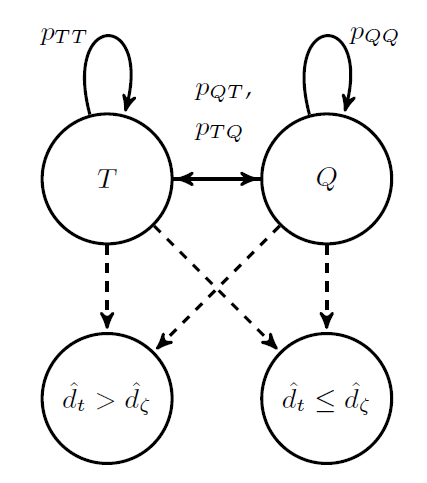
\includegraphics[width=5.93in]{quiet_turb_hmm} 

}

\caption{Turbulent / quiet hidden Markov model.}\label{fig:hmm}
\end{figure}

The transition matrix stores the probabilities of transition from a state at time \(t\) to another at
time \(t + 1\) for ease of computation. It is mathematically shown as:
\[P_{t, t + 1} = \begin{bmatrix} 
p_{QQ} & p_{QT} \\
p_{TQ} & p_{TT}  
\end{bmatrix},\]
where the matrix applies to all times \(t\). Because the matrix applies to all times the system is called
stationary, and the long-run probabilities of being in each state will converge. Once we have
determined the most likely state at time \(t\) using an algorithm such as the Viterbi algorithm, we can
use the series of estimated states \(\{\hat{s}_t: t \in \{0, 1, ..., T\}\}\) to partition the
data history. The two datasets would be data used for the quiet sample covariance matrix and data used
for the turbulent sample covariance matrix. \citet{FD18} blend these two sample matrices using the investor's
risk preferences and the most recent probabilities of being in each state, yielding a more
sophisticated estimator of \(\Sigma\).

An alternative approach to dealing with heterogeneity is to focus on the assumption that errors for
return forecasting models have a normal distribution. But first, we need to define a general return
forecasting model. If the return of a portfolio is viewed through a set of return drivers or risk
factors, then returns could be explained in part by those factors and the portfolio's sensitivity to
them. \citet{M10} encapsulates this idea in his asset return model given below:
\begin{align}
R &= \alpha +\beta^\intercal \mathcal{F} + \epsilon, \label{eq:retfact}
\end{align}
where \(R\) is a vector of asset returns (not portfolio returns through time as shown previously),
\(\alpha\) is a forecastable vector of returns unique to each security, \(\beta\) is a matrix of
sensitivities to risk factors, \(\mathcal{F}\) is a vector of factors, and \(\epsilon\) is the error
vector. The error vector is assumed to have a normal distribution. \citet{AC02} show that in a downward
market, the correlation structure is significantly different from what is implied by a normal
distribution, which is a problem when using model \eqref{eq:retfact} in the exhibited way. \citet{CDG19}
address the issue of non-normal errors by utilising the quantile regression model proposed by
\citet{KB78}. The asset returns, idiosyncratic asset returns, asset factor sensitivities and errors could all
be considered to be a function of the current quantile, denoted \(\tau\). This leads to the quantile
factor model (QFM):
\begin{align} 
\mathcal{Q}(\tau) =  \alpha(\tau) + \beta(\tau)\mathcal{F} + \epsilon(\tau), \label{eq:qfm}
\end{align}
where \(\tau \in [0, 1]\). In a different symmetric, normally distributed world, \(\tau\) can be set to
\(0.5\) and model \eqref{eq:retfact} will be recovered. However, in the real world where symmetry and
normality are often not adhered to, the quantile conditional errors can be defined more generally so
that they only have to satisfy:
\begin{align}
\mathbb{P}\Big[\epsilon(\tau) \leq \underline{0} \, \Big | \mathcal{F} \Big] = \tau \; .
\end{align}
This structure emerges from the cumulative distribution function (CDF) conditional on the set of
factors of each asset return \(R_i\). Given the conditional CDF for the returns on asset \(i\),
\(F_i(R_i|\mathcal{F})\), the quantile specific inverse CDF, \(F^{-1}_i(\tau| \mathcal{F})\), can be used
to generate the quantiles \(\mathcal{Q}_i(\tau)\). \citet{FD18} suggest using the information about each
quantile to construct a series of quantile-specific covariance matrices, which can then be blended to
yield a more sophisticated estimator of \(\Sigma\). Chapter \textbf{insert ref to next chapter} covers the
implementations of these two techniques to better estimate \(\Sigma\).

\hypertarget{penalising-the-optimization}{%
\subsection{Penalising the optimization}\label{penalising-the-optimization}}

To add a penalty term in a way that preserves the goal of the risk optimisation, we first need to
adapt the objective functions of each risk-based portfolio as given earlier in chapter
@ref\{rbportch\}. Consider the return-targeting penalised optimisation approach of \citet{K18}, both choices
of \(f(\cdot|\textbf{X})\) for the GMV and ERC portfolios can be adapted into this approach. Beginning
with the GMV portfolio, Kinn views the portfolio variance as an expectation:
\begin{align*}
f(w, \Sigma  | \textbf{X}) &= w^\intercal \Sigma w &\\
& = w^\intercal (\mathbb{E}[{r}_t {r}_t^\intercal] - \mu \mu^\intercal) w & \small\text{(alternate definition of $\Sigma$)} \\
& = \mathbb{E}[|w^\intercal \mu - w^\intercal {r}_t|^2],
\end{align*}
where \({r}_t\) represents the asset returns above the risk-free rate, and \(\mu\) is a vector of the
population expected excess returns as before. Rewriting the portfolio expected excess return as
\(\bar{r} = w^\intercal \mu\), the idea of return-targeting for a portfolio can be incorporated as the
expectation of \(|\bar{r} - w^\intercal {r}_t|^2\), which is the squared distance to a target return
level. Kinn's approach is consistent with an MVO optimisation intuitively because the target return
level is analogous an expected return constraint and minimising the return's squared distance to this
constraint is analogous to variance minimisation. The objective function can now be approximated using
the sample average as a result of the law of large numbers. We still have to show how to find the GMV
portfolio from an MVO procedure. As stated in table \ref{tab:rbportprops}, the GMV portfolio is the
MSR portfolio if the assumption of identical excess returns is met. Therefore, if the target return is
set to a value that is easily obtainable \(\bar{r} = \bar{r}_\mathrm{gmv}\), then the scheme will yield
a GMV portfolio. This easily obtainable value has to be found numerically and cannot be determined a
priori. The non-rigorous argument turns out to be empirically true for the portfolios analysed in this
research. When the return vector is replaced by the set of sample returns \(\textbf{X}\), and the
expectation is approximated by the sample average, the \citet{K18} form of objective function is recovered:
\begin{align}
f_{\text{Kinn}}(w|\textbf{X}) &= \frac{1}{T} \sum_{t = 1}^T  (\bar{r}_\mathrm{gmv} - \textbf{X}^\intercal_t w)^2, \label{eq:kinnop1}
\end{align}
where \(t\) indexes columns of the sample returns matrix \(\textbf{X}\). The GMV portfolio can be found equivalently in this way.

The log-constraint\footnote{The log-constraint is also introduced in appendix \textbf{insert appendix ref}.},
\(\sum_i \ln(w_i) \geq c\), can be placed on optimisation \eqref{eq:kinnop1} to recover the ERC
portfolio. To include the constraint in framework \eqref{eq:genopt}, a Lagrangian multiplier approach
can be used to move the log-constraint to the objective function. Kinn's adapted ERC objective
function is then:
\begin{align}
f_{\text{Kinn}}(w|\textbf{X}) &= \frac{1}{T} \sum_{t = 1}^T  (\bar{r}_{gmv} - \textbf{X}^\intercal_t w)^2 -\eta_{erc}\sum_{i = 1}^N \ln(w_i),
\end{align}
where \(\eta_{erc}\) is the Lagrangian multiplier scalar. Now that we have shown the standard objective
functions from earlier are equivalent to the Kinn framework, we have also vindicated the general
framework \eqref{eq:genopt} as accommodative of a valid application of supervised machine learning
(SML) to portfolio optimisation.

Because logical choices for \(f_{\text{Kinn}}(\cdot|\textbf{X})\) have been established, different
penalty functions can be applied to the optimisation. Two common penalised regression techniques are
lasso regression and ridge regression (RR). In the presence of a long-only constraint, as is applied
in this research, a lasso regression does not make sense, because the penalty function is simply the
sum of the absolute weights: \(P(w) = \sum_{i= 1}^N |w_i| =1\). This penalty is equal to \(1\) for all
constrained portfolios. Separately, the RR is obtained by specifying the penalty as the sum of squares
for the portfolio weights: \(P(w) = \sum_{i= 1}^N w_i^2\). The penalty reduces the number of admissable
concentrated portfolios and intuitively is not unlike incorporating some of the EW portfolio into the
ERC or GMV portfolios. Ignoring constraints, \citet{LW04} show that RR has the same effect as shrinking
the sample covariance matrix towards the identity matrix for the GMV optimisation:
\begin{align}
\textbf{S}_{RR} = \textbf{S} + \frac{\lambda}{T} \textbf{I}, 
\end{align}
where \(\lambda\) is the shrinkage intensity, and \(T\) is the number of sample observations. In the
presence of constraints, the actual scaling factor is slightly different from Ledoit and Wolf's
calculations, but the intuition of shrinkage towards the identity matrix still applies. If \(\lambda\)
becomes very large, the minimum variance portfolio will tend towards the EW portfolio. Estimating
lambda is thus a practical choice, and the process to do so consistently is outlined in the next
chapter.

\hypertarget{alternate-implementation-methods}{%
\subsection{Alternate implementation methods}\label{alternate-implementation-methods}}

\citet{SW17} present a means to find a resampled MVO portfolio that reduces estimation risk by optimising
random subsets of assets in the investment universe. The process is called subset resampling (SRS).
They then aggregate resultant optimised subset portfolios to create a final `optimal' solution. The
procedure requires the inputs of a sample return matrix \(\textbf{X}\) and an asset subset size \(b\).
The subset size is related to the extent of the trade-off between bias and variance. We have to
choose the degree of repeated sampling, \(s\), which is restricted by the available computational
power.

This method can be described as follows. For each of the \(s\) repeated samples, we randomly select
the \(j^{\text{th}}\) subset of \(b\) assets from the \(N\) assets in the investment universe, denoted
\(\mathcal{I}_j\). Using only the sample return data from the selected asset subset \(\textbf{X}_j\), we
then compute the associated optimal portfolios \(\hat{w}_j\) using framework \eqref{eq:genopt} and a
given choice of objective function. Finally, we average the \(s\) optimal subset weight vectors to
obtain the final optimal asset portfolio \(\hat{w}_\mathrm{srs} = (\sum_{j = 1}^s \hat{w}_j)s^{-1}\).

The SRS process is very general, and could even be applied in conjunction with a penalised
optimisation or an improved sample covariance matrix. Additionally, the user can choose the input
\(b\). If \(b = N\), then the usual sample risk-based portfolio is recovered, albeit in a
computationally expensive manner. If \(b = 1\), then the SRS procedure will yield the EW portfolio for
a large enough value of \(s\). Therefore, \(b\) is the input parameter controlling the extent of the
trade-off between weight diversification and estimation risk. The estimation of \(b\) should be done
in a manner consistent with the aim of the optimisation. To ensure \(b\) scales with the size of the
asset universe, \citet{SW17} recommend writing it in the form \(b = N^{\alpha}\), where \(\alpha \in [0, 1]\).

The SRS method is comparable to ensemble methods in machine learning. The logical basis is that many
different models can be used and aggregated into a final model, rather than assuming a single model
is the most accurate to use. Despite the general nature of the SRS procedure, it is still consistent
with the approach of increasing the squared bias out of the hope that the variance reduction will
offset it enough to lessen overall estimation risk.

Each of the three estimation risk reduction classes has at least one specific technique within them.
Some modelling decisions need to be made for a prospective user to apply these techniques in an
experiment. These modelling decisions are covered in the next chapter.

\hypertarget{somemaths}{%
\section{Using estimation risk reduction techniques}\label{somemaths}}

Under the EW and MW portfolios, the portfolio weights do not require estimation whereas the GMV and ERC
portfolios do. For each of these portfolios, there are six given ways of performing the estimation in
this research. The first is by using the standard sample covariance matrix, the next four are to use
techniques outlined in chapter \ref{estriskreduce}, and the final one is to use a combination of
quantile factor modelling and regime switching. A summary of all of the portfolio technique pairs is
given in table \ref{tab:portestpairs} below.

\begin{longtable}[]{@{}lll@{}}
\caption{\label{tab:portestpairs} Portfolio estimation-technique pairs}\tabularnewline
\toprule
\begin{minipage}[b]{0.27\columnwidth}\raggedright
Portfolio\strut
\end{minipage} & \begin{minipage}[b]{0.50\columnwidth}\raggedright
Estimation technique\strut
\end{minipage} & \begin{minipage}[b]{0.14\columnwidth}\raggedright
Abbreviation\strut
\end{minipage}\tabularnewline
\midrule
\endfirsthead
\toprule
\begin{minipage}[b]{0.27\columnwidth}\raggedright
Portfolio\strut
\end{minipage} & \begin{minipage}[b]{0.50\columnwidth}\raggedright
Estimation technique\strut
\end{minipage} & \begin{minipage}[b]{0.14\columnwidth}\raggedright
Abbreviation\strut
\end{minipage}\tabularnewline
\midrule
\endhead
\begin{minipage}[t]{0.27\columnwidth}\raggedright
Equal weight\strut
\end{minipage} & \begin{minipage}[t]{0.50\columnwidth}\raggedright
-\strut
\end{minipage} & \begin{minipage}[t]{0.14\columnwidth}\raggedright
EW\strut
\end{minipage}\tabularnewline
\begin{minipage}[t]{0.27\columnwidth}\raggedright
Market weight\strut
\end{minipage} & \begin{minipage}[t]{0.50\columnwidth}\raggedright
-\strut
\end{minipage} & \begin{minipage}[t]{0.14\columnwidth}\raggedright
MW\strut
\end{minipage}\tabularnewline
\begin{minipage}[t]{0.27\columnwidth}\raggedright
Global minimum variance\strut
\end{minipage} & \begin{minipage}[t]{0.50\columnwidth}\raggedright
Sample covariance matrix\strut
\end{minipage} & \begin{minipage}[t]{0.14\columnwidth}\raggedright
GMV-SCM\strut
\end{minipage}\tabularnewline
\begin{minipage}[t]{0.27\columnwidth}\raggedright
Global minimum variance\strut
\end{minipage} & \begin{minipage}[t]{0.50\columnwidth}\raggedright
Quantile factor modelling\strut
\end{minipage} & \begin{minipage}[t]{0.14\columnwidth}\raggedright
GMV-QFM\strut
\end{minipage}\tabularnewline
\begin{minipage}[t]{0.27\columnwidth}\raggedright
Global minimum variance\strut
\end{minipage} & \begin{minipage}[t]{0.50\columnwidth}\raggedright
Regime switching\strut
\end{minipage} & \begin{minipage}[t]{0.14\columnwidth}\raggedright
GMV-RS\strut
\end{minipage}\tabularnewline
\begin{minipage}[t]{0.27\columnwidth}\raggedright
Global minimum variance\strut
\end{minipage} & \begin{minipage}[t]{0.50\columnwidth}\raggedright
Quantile factor modelling with regime switching\strut
\end{minipage} & \begin{minipage}[t]{0.14\columnwidth}\raggedright
GMV-QRS\strut
\end{minipage}\tabularnewline
\begin{minipage}[t]{0.27\columnwidth}\raggedright
Global minimum variance\strut
\end{minipage} & \begin{minipage}[t]{0.50\columnwidth}\raggedright
Ridge regression\strut
\end{minipage} & \begin{minipage}[t]{0.14\columnwidth}\raggedright
GMV-RR\strut
\end{minipage}\tabularnewline
\begin{minipage}[t]{0.27\columnwidth}\raggedright
Global minimum variance\strut
\end{minipage} & \begin{minipage}[t]{0.50\columnwidth}\raggedright
Subset re-sampling\strut
\end{minipage} & \begin{minipage}[t]{0.14\columnwidth}\raggedright
GMV-SRS\strut
\end{minipage}\tabularnewline
\begin{minipage}[t]{0.27\columnwidth}\raggedright
Equal risk contribution\strut
\end{minipage} & \begin{minipage}[t]{0.50\columnwidth}\raggedright
Sample covariance matrix\strut
\end{minipage} & \begin{minipage}[t]{0.14\columnwidth}\raggedright
ERC-SCM\strut
\end{minipage}\tabularnewline
\begin{minipage}[t]{0.27\columnwidth}\raggedright
Equal risk contribution\strut
\end{minipage} & \begin{minipage}[t]{0.50\columnwidth}\raggedright
Quantile factor modelling\strut
\end{minipage} & \begin{minipage}[t]{0.14\columnwidth}\raggedright
ERC-QFM\strut
\end{minipage}\tabularnewline
\begin{minipage}[t]{0.27\columnwidth}\raggedright
Equal risk contribution\strut
\end{minipage} & \begin{minipage}[t]{0.50\columnwidth}\raggedright
Regime switching\strut
\end{minipage} & \begin{minipage}[t]{0.14\columnwidth}\raggedright
ERC-RS\strut
\end{minipage}\tabularnewline
\begin{minipage}[t]{0.27\columnwidth}\raggedright
Equal risk contribution\strut
\end{minipage} & \begin{minipage}[t]{0.50\columnwidth}\raggedright
Quantile factor modelling with regime switching\strut
\end{minipage} & \begin{minipage}[t]{0.14\columnwidth}\raggedright
ERC-QRS\strut
\end{minipage}\tabularnewline
\begin{minipage}[t]{0.27\columnwidth}\raggedright
Equal risk contribution\strut
\end{minipage} & \begin{minipage}[t]{0.50\columnwidth}\raggedright
Ridge regression\strut
\end{minipage} & \begin{minipage}[t]{0.14\columnwidth}\raggedright
ERC-RR\strut
\end{minipage}\tabularnewline
\begin{minipage}[t]{0.27\columnwidth}\raggedright
Equal risk contribution\strut
\end{minipage} & \begin{minipage}[t]{0.50\columnwidth}\raggedright
Subset re-sampling\strut
\end{minipage} & \begin{minipage}[t]{0.14\columnwidth}\raggedright
ERC-SRS\strut
\end{minipage}\tabularnewline
\bottomrule
\end{longtable}

\hypertarget{quantile-factor-modelling-and-regime-switching}{%
\subsection{Quantile factor modelling and regime switching}\label{quantile-factor-modelling-and-regime-switching}}

QFM and RS improve the estimation of the inputs into the optimisation and therefore have the same
implementation for the GMV and ERC portfolios. To use the RS model for covariance prediction, the
probability of being in either a quiet or a turbulent state needs to be estimated. If \(s_t\) is the
random variable that takes on the value of the state at time \(t\) then \(s_t \in \{Q, T\}\). The true
parameters are defined as:
\begin{align*}
\pi_{Q, t} &:= \mathbb{P}\{s_t = Q\}, \\
\pi_{T, t} &:= \mathbb{P}\{s_t = T\} = 1 - \pi_{Q, t}.
\end{align*}
These can be estimated using the emission quantities from the HMM, \(\hat{d}_t\), and a maximum
likelihood approach - the Baum-Welch algorithm\footnote{An influential tutorial on this algorithm and
  HMMs was given by \citet{R89}.}. \citet{K12} determine a turbulent-quiet data split through the parameter \(\zeta\),
which is the proportion of the data allocated to the quiet regime for covariance estimation. They
suggest a value of \(0.7\) or \(0.8\), but due to constraints on input data length we use \(0.7\) in this
research. The investor has nearly estimated enough parameters to blend the variance-covariance matrix
using the method of \citet{FD18} outlined below in equation \eqref{eq:fdblend}.
\begin{align}
\hat{\Sigma}_{\text{blend}} & = \hat{\pi}_{Q, t + 1} \hat{\eta}_Q \hat{\Sigma}_Q + \hat{\pi}_{T, t + 1} \hat{\eta}_T \hat{\Sigma}_T. \label{eq:fdblend}
\end{align}
The estimated probabilities, \(\hat{\pi}_{Q, t + 1}\) and \(\hat{\pi}_{T, t + 1}\), are forward-looking.
Predictions can be made empirically using the current state because the transition probabilities are
generally near \(1\) or \(0\) in the data. The investor still has to estimate their normalised aversion to
each regime \(\hat{\eta}_{s_{t+1}}\), which they can do using the estimation procedure from \citet{B18}. For
the experiment, the investor was indifferent between regimes.

The intention of this blending procedure is for money managers to estimate the state probabilities
themselves, thus incorporating their future beliefs. In reality, when implementing a quantitative
model, it is common to use a rolling estimation window of data. Asset return data is often not long
enough to accommodate sophisticated portfolio construction methods. Therefore, assigning
\(\hat{\pi}_{T, t + 1}\) values near \(1\) results in the estimation and application of large covariance
matrices with potentially only \(30 \%\) of the data, without the requisite weighting of the other
covariance matrix. The inaccurate covariance matrix leads to the very same input sensitivity problems
that the RS model attempts to avoid. It is worth clarifying that the sensitivity is due to an
incorrectly estimated \(\hat{\pi}_{T, t + 1}\), not the absence of underlying regimes. To correct this
sensitivity concern, a discretised simplification is used. If the state is estimated to be quiet,
nothing is done to the weights implied by the volume of data:
\begin{align*}
(\hat{\pi}_{Q, t + 1}, \hat{\pi}_{T, t + 1}) = (\zeta, 1 - \zeta).
\end{align*}
If the state is estimated to be turbulent, then the weights implied by the volume of data are adjusted
to overweight the turbulent regime by a proportion of \(\gamma\):

\begin{align*}
(\hat{\pi}_{Q, t + 1}, \hat{\pi}_{T, t + 1}) = (\zeta -  \frac{\gamma}{2}, 1 - \zeta + \frac{\gamma}{2}).
\end{align*}
In the experiment, we set \(\gamma\) to 0.1. The effect is that in the quiet regime, the covariance
matrix is the same as without the RS model. While during the turbulent regime, the turbulent covariance
matrix is given a weighting of \(\gamma\) more than what is implied by the data split.

The QFM technique is examined next. \citet{CDG19} use the QFM technique from equation \eqref{eq:qfm} for
prediction. They select risk factors and estimate factor loadings using a simultaneous procedure.
Factor-based modelling is not the focus of this research, although it can be used in conjunction with
the general framework \eqref{eq:genopt}. In this experiment, mainly for pedagogical purposes, simple
factors are used for the QFM portfolios; namely, a market factor and a squared market factor. This
choice is consistent with the findings of \citet{TM66}, with more detail given in appendix
\textbf{insert appendix reference here}. Additionally, the QFM user has to choose how to partition the
interval \([0, 1]\), i.e.~decide which quantiles to use. The partition is an important input which could
be estimated. We use the same split as \citet{MP08}\}, where: \[[\tau_0 = 0, \tau_1 = 0.1]\cup(\tau_1 = 0.1,
\tau_2 = 0.9] \cup (\tau_2 = 0.9, \tau_3 = 1].\] In the notation, the intervals are referred to by
their right endpoint. \citet{FD18} note that the QFM, as stated, does not provide variation between
quantiles, as the idiosyncratic error term will always adjust so that the total estimated covariance
matrix is always equal to the sample covariance matrix. Therefore, to estimate the quantile specific
covariance matrices, they propose fixing the error term to the median error such that
\(\hat{\epsilon}(\tau) = \hat{\epsilon}(0.5)\). Then each set of quantile returns can be used to
construct a sample covariance matrix denoted \(\hat{\Sigma}^{(\tau)}\). \citet{MP08} propose a strategy for
portfolio forecasting called quantile regression portfolio distribution (QRPD). It involves
interval-weighting the portfolio allocations \(\hat{w}^{(\tau)}\) for each quantile covariance matrix.
The QRPD portfolio is:
\begin{align}
\hat{w}_{\text{QRPD}} & = \sum_{i = 1}^{l} p_i\hat{w}^{(\tau_i)},\;\;
\end{align}
where \(p_i = \tau_i - \tau_{i - 1}\), and \(l\) is the number of intervals. Like the SRS method, the QRPD
method is comparable to ensemble methods because different models are being aggregated in the hope of
reducing total estimation risk.

The QRS technique from table \ref{tab:portestpairs} is laid out by \citet{FD18}. They first separate the
data history into regimes. Within each regime, they apply the QFM approach. Once they find
\(\hat{\Sigma}_{s_t}^{(\tau_i)}\) for every quantile and state, they blend the covariance matrices
between regimes. For every possible pair of quantiles
\(\tau_i, \tau_j \in \{\tau_1, ..., \tau_{|\tau|}\}\), a blended SCM can be constructed:
\begin{align}
\hat{\Sigma}^{(\tau_i, \tau_j)}_{\text{blend}} & = (\hat{\pi}_{Q, t  + 1}\hat{\eta}_Q\hat{\Sigma}^{(\tau_i)}_Q) + (\hat{\pi}_{T, t  + 1}\hat{\eta}_T\hat{\Sigma}^{(\tau_j)}_T).
\end{align}
Each of the SCMs can be used to find a portfolio \(\hat{w}^{(\tau_i, \tau_j)}\). Once the \(l \times l\)
portfolios have been found they can also be blended with the QRPD method:
\begin{align}
\hat{w}_{\text{QRPD}} & =  \sum_{i = 1}^{|\tau|}  \sum_{j = 1}^{|\tau|} p_i p_j \hat{w}^{(\tau_i, \tau_j)}.
\end{align}

\hypertarget{ridge-regression}{%
\subsection{Ridge regression}\label{ridge-regression}}

As stated previously, the QFM and RS techniques do not require separate workarounds for the ERC and
GMV portfolios. This is not the case for the RR method. First, we consider the GMV portfolio
estimation and then the ERC portfolio estimation. The Lagrangian multiplier, \(\lambda\), for the
penalty in framework \eqref{eq:genopt}, should be chosen to minimise the estimation risk. However, the
estimation risk is unobservable. \citet{K18} suggests the k-folds cross-validation estimation procedure to
select this parameter\footnote{The procedure is outlined by \citet{FHT01}.}. The broad idea of this procedure is to
approximate the estimation risk and choose a value of lambda, \(\lambda^*\), that minimises the
approximated estimation risk. To perform k-folds cross-validation, we initially arrange the
observations into \(K\) subsets without replacement. The subsets are taken over time and not assets as
with SRS technique. The set of observations for the \(k^{\text{th}}\) subset is denoted \(\mathcal{I}_k\).
All of the observations in the \(K - 1\) remaining subsets (i.e.~excluding those in the \(k^{\text{th}}\)
subset) are stored in a set denoted \(\mathcal{I}_{-k}\). This yields the optimisation:
\begin{align}  
\lambda^* & = \underset{\lambda}{\text{argmin}} \Big \{ \frac{1}{K} \sum_{k =1}^K \hat{h}_k(\lambda, \mathcal{I}_k, \mathcal{I}_{-k})\Big \}, \label{eq:scorefunc}
\end{align}
where \(\hat{h}_k(\lambda)\) is a function that approximates estimation risk given a value of \(\lambda\).
One choice for \(h\) is the mean squared error penalty for a portfolio found using the data from
\(\mathcal{I}_{-k}\) and then tested on \(\mathcal{I}_k\). This procedure is described below:

\begin{enumerate}
\def\labelenumi{\arabic{enumi}.}
\item
  For each subset \(k = \{1, 2, ..., K\}\), find the optimal portfolio weights using the training data \(\mathcal{I}_{-k}\) and apply the penalty scaled by \(\lambda\).
\item
  Evaluate the performance of this portfolio on the unused data \(\mathcal{I}_k\) with the mean squared error loss function and retain the score \(\hat{h}_k\):
  \begin{align}
  \hat{h}_k (\lambda, \mathcal{I}_k, \mathcal{I}_{-k}) = \frac{1}{|\mathcal{I}_k|} \sum_{i \in \mathcal{I}_k} (\bar{r}_{gmv} - \textbf{X}_i^\intercal \hat{w}_{\mathcal{I}_{-k}}(\lambda))^2, \label{eq:hfunc}
  \end{align}
  where \(\bar{r}_{gmv}\) is determined as in chapter \ref{estriskreduce}, and the function \(|\cdot|\)
  counts the number of observations in a set.
\item
  The range of possible \(\lambda\) values can be discretised to find a solution that minimises the
  objective function in \eqref{eq:scorefunc}\footnote{The objective function in \eqref{eq:scorefunc} can
    be computationally expensive to evaluate; hence, an efficient approximation procedure is necessary.}.
\end{enumerate}

For the ERC portfolio implementation of the RR method, there is an additional hyperparameter,
\(\eta_{erc}\), that needs to be estimated. This hyperparameter should be found before the penalty
hyperparameter \(\lambda^*\). We also use the k-folds cross-validation technique to find this parameter.
However, the mean squared error loss to the desired global minimum variance portfolio from equation
\eqref{eq:hfunc} is not appropriate for optimising an ERC portfolio. Ideally, \(\eta_{erc}^*\) should
minimise the distance between all of the total risk contributions so that they are as equal as
possible. Therefore, we make use of the following hyperparameter selection function (see appendix
\textbf{insert reference to appendix here} for motivation):
\begin{align}
\hat{h}_k^{erc} (\eta, \mathcal{I}_k, \mathcal{I}_{-k}) & = \sum_{i = 1}^N  \sum_{j \geq i}^N(\hat{w}_{i, \mathcal{I}_{-k}}(\textbf{S}_{\mathcal{I}_k} \hat{w}_{\mathcal{I}_{-k}})_i - \hat{w}_{j, \mathcal{I}_{-k}}(\textbf{S}_{\mathcal{I}_k} \hat{w}_{\mathcal{I}_{-k}})_j )^2.
\end{align}

\hypertarget{experiment}{%
\section{An empirical test using Sourth African equities}\label{experiment}}

In this chapter, we test the various approaches outlined above for constructing risk-based portfolios
using South African equity data. There are two sources of variation in this experiment: variation in
risk-based portfolio type and variation in estimation risk reduction technique, all combinations of
which are outlined in table \ref{tab:portestpairs}. Each combination of portfolio-technique approach
will be referred to as a pair.

\hypertarget{data-and-methodology}{%
\subsection{Data and methodology}\label{data-and-methodology}}

The available data for this experiment are weekly total-returns for all equity stocks included in the
Johannesburg Stock Exchange (JSE) All Share Index (ALSI) over the period ranging from the \(5^{th}\)
January 1996 to the \(1^{st}\) November 2019. Weightings of the shares in the ALSI are also available,
although this is a monthly series. This historical vector of the weights of the MW portfolio through
time is denoted \(\hat{w}^{\text{mw}}_t\).

The investigation uses a rolling estimation window of \(T = 400\)\footnote{\(400\) weeks or \(7.69\) years
  may seem like an odd choice. It is a window that balances the need for enough estimation data, but also
  a lengthy out-of-sample test. For a longer data history, a larger estimation window could be used.}
weekly observations to construct portfolios. Weekly data inputs are used with monthly rebalancing
because of the high data volume requirement from chapter \ref{somemaths}. The constructed portfolio
\(\hat{w}_{t_i}\) will be held out-of-sample over the interval \([t_i, t_{i + 1}]\), where \(t_i\) denotes a
month's end. The entire holding period is from the \(30^{th}\) of September 2003 to the \(27^{th}\) of
September 2019 a total of 16 years. Portfolios are constructed for two different asset universes;
namely, the \(40\) largest stocks and the \(100\) largest stocks. The separation is to test the effect on
portfolio performance of an investor broadening their universe. This methodology is outlined for each
rebalancing date:

\begin{enumerate}
\def\labelenumi{\arabic{enumi}.}
\item
  Of the stocks in the ALSI with a data history of at least length \(T\), choose the \(N\) stocks with the
  largest market weights.
\item
  Use the \(N \times T\) matrix of sample returns to find asset weights for the relevant
  portfolio-technique pair.
\item
  Hold the found portfolio \(\hat{w}\) for one month, record the returns \(\hat{r}\), and calculate the
  portfolio turnover.
\end{enumerate}

This experiment is specific to this data and method. Therefore, it is important to outline some
limitations of the results. Although framework \eqref{eq:genopt} is broad, this experiment only analyses
portfolios constructed with South African equity returns, and cannot be used to state facts about the
portfolio construction process generally. The budget, long-only and maximum weight constraints were all
applied for this experiment. Specifically the maximum weight constraint used is \(\alpha = 0.1\). The
choice intends to provide a consistent basis for comparison across portfolio-technique pairs and
ensures similarity to practical applications. Shares that have missing data were excluded at each
rebalancing date with a filter, therefore the MW portfolio, where \(N = 40\) may not be representative of
the JSE Top 40 index. Transaction costs are ignored due to the liquid nature of the largest stocks,
although this is a potential area for future improvement on the backtesting methodology.

\hypertarget{results}{%
\subsection{Results}\label{results}}

Before the results are reported, specific metrics that illustrate the effect of each technique and
portfolio need to be introduced. The first is turnover (TO). It measures the magnitude of trading
required on each rebalancing date. If there are \(m\) rebalancing dates, then the TO is calculated as:
\begin{align}
\text{TO} & = \frac{6}{(m - 1)} \sum_{i = 1}^{m - 1} \sum_{j =1}^{N} |\hat{w}_{t_i, j}^\triangle - \hat{w}_{t_i, j}|,
\end{align}
where \(\hat{w}_{t_i, j}^\triangle\) is the buy-and-hold weight of the \(j^{th}\) asset just before the
rebalance at time \(t_i\). The turnover is annual and one-way only; hence, the scaling factor of
\(\frac{6}{m-1}\). For a higher TO, the investor has increased risk when rebalancing that they will not
enter into the new portfolio at the current market price. The maximum possible value of the TO is
\(1200\%\), and the investor achieves it if they switch from one single stock portfolio to another at
every rebalancing date.

The next reporting metric is maximum drawdown (MDD), the definition of which requires the notion of
cumulative wealth. The investor's cumulative wealth at time \(t_j\) is their return from time \(t_0\)
until time \(t_j\) on a portfolio of one initial unit investment, and it is defined as:
\begin{align*}
W_{t_j} &= \prod_{i = 1}^{j} (1 + \hat{r}_{t_i}), 
\end{align*}
where \(\hat{r}_{t_i}\) is the return realised over the interval \([t_{i - 1}, t_i)\). The MDD is the
biggest loss in cumulative wealth for the entire investment period, and is formulated as:
\begin{align}
\text{MDD} & = \underset{t_j \in \{t_1, ..., t_m\}}{\text{argmax}} \Big \{ \underset{t_i \in \{t_1, \text{...}, t_j\}}{\text{argmax} \{W_{t_i} \}} - W_{t_j}  \Big \} \; .
\end{align}
MDD is an essential measure for money managers because excessive drawdowns lead to redemptions in
their funds. \citep{M04}

The last two measures are measures of concentration. As stated earlier, the risk-based investor is
making a trade-off between weight concentration and risk concentration. A standard for weight
concentration at a rebalancing date, the inverse Herfindahl index, has already been defined. But the
IHI is general and could apply to multiple types of weights. For allocation weights the IHI at time
\(t_i\) is given as:
\begin{align}
N^{\text{eff}}_{t_i} &= \frac{1}{\sum_{j = 1}^N w_{t_i, j}^2} \; ,
\end{align}
where \$N\^{}\{\text{eff}\}\emph{\{t\_i\} \$ can be interpreted as the number of equal-weighted stocks the investor's
portfolio is equivalent to. The notation reflects the idea that the IHI represents the number of
effective stocks in the portfolio. The upper bound of \$N\^{}\{\text{eff}\}}\{t\_i\} \$ is \(N\) and the lower
bound in the presence of a maximum allocation constraint is:
\(({\lfloor \frac{1}{\alpha} \rfloor \cdot \alpha^2 + (1- \lfloor \frac{1}{\alpha}\rfloor \cdot \alpha)^2})^{-1}\)
, which is derived in appendix \ref{ihimax}. For the case when \(\alpha = 0.1\) the lower bound is
\(10\). Risk-weights can be taken instead of capital weights to measure the effectiveness of an asset on
portfolio volatility. Since the TRCs sum to the portfolio volatility, the risk contributions can be
scaled into risk-weights so that they sum to \(1\). The risk-weight for the \(j^{th}\) asset at time \(t_i\)
is given as:
\begin{align}
\text{RW}_{t_i, j} &= \frac{\text{TRC}_{t_i, j}}{\sqrt{w_{t_i}^\intercal \Sigma w_{t_i}}}\; ,
 \end{align}
where the inverse Herfindahl index approach can be applied again. The risk-weight IHI is written as:
\begin{align}
N^\mathrm{rw}_{t_i}(RW_{t_i}) &= \frac{1}{\sum_{j = 1}^N \text{RW}_{t_i, j}^2} \;.
\end{align}
If \(\Sigma\) is positive semi-definite, then the lower bound is \(1\) even in the presence of the maximum
allocation constraint, because one asset could have a positive weight and considerable volatility. The
upper bound is once again \(N\). The concentration measures are reported as averages across all of the
\(m\) rebalancing dates.

Let us first discuss the results for the GMV portfolios. The main objective of constructing GMV
portfolios is to reduce the out-of-sample volatility of returns. The main aim of each GMV-technique
pair is the same, but performance is measured against the GMV-SCM pair. Therefore, it makes sense to
define a measure of each GMV-technique pair performance in the same way as \citet{RR15}, as a
volatility reduction over the GMV-SCM pair:
\begin{align}
\mathcal{VR}(w|w_{\text{gmv-scm}}) & = \frac{\sigma(w_{\text{gmv-scm}}) - \sigma(w)}{\sigma(w_{\text{gmv-scm}})},
\end{align}
where the \(\sigma(\cdot)\) function measures a portfolio's volatility.

\hypertarget{going-to-rify}{%
\subsubsection{going to R'ify}\label{going-to-rify}}

\hypertarget{conclusion}{%
\section{Conclusion}\label{conclusion}}

This dissertation introduces a flexible framework for risk-based investing that is a general tool and
allows the user to incorporate different estimation techniques into their risk-based portfolio
construction. The framework and risk-based investing are empirically sound when tested with South African
data, as all risk-based portfolios outperformed the market weight portfolio using the Sharpe ratio
measure. The superiority of risk-based portfolios is consistent with similar results for US equities
found by \citet{DGL07} and \citet{K10}.

Within risk-based portfolios, we found that GMV portfolios performed the best using the same Sharpe ratio
measure. Furthermore, broadening the asset universe to include more assets materially improved portfolio
performance.

No techniques outperformed the standard sample covariance matrix technique for finding risk-based
portfolios across all risk-based portfolios, which is consistent with the findings of \citet{K10}. However,
they propose longer estimation windows (20-years or 10-years) than were used in this study. Due to the
similar performance of shrinkage techniques and standard sample estimation techniques, the period of this
study (7.69-years) is close to an empirical break-even performance point between sample estimation and
lack-of-data adjusted estimation strategies.

Quantile factor modelling with regime switching worked well for the smaller and more concentrated GMV
portfolios, where estimating a small number of substantial allocations correctly is essential. Subset
resampling performed well for the less concentrated ERC portfolios, where determining the greatest number
of allocations is necessary. Ridge regression shrinkage techniques have historically performed well in
other studies. Still, the long-only constraint and a restrictive maximum allocation constraint of 10\%
have the effect of regularising the optimisation in a manner already shown by JM03. Therefore, the
impact of ridge regression on performance is diminished.

\hypertarget{avenues-for-further-research}{%
\subsection{Avenues for further research}\label{avenues-for-further-research}}

Avenues for further research include using the flexible investing framework with other risk-based
portfolios and penalising the objective function with alternate functions. The structure may also be
modified to include different constraints. Further experiments may also be performed with varying
universes of assets. Additionally, the general portfolio estimation procedure could be performed in
risk factor space instead of the asset space.

\hypertarget{appendix-appendix}{%
\appendix}


\hypertarget{abbreviations}{%
\section{Abbreviations}\label{abbreviations}}

\begin{longtable}[]{@{}ll@{}}
\caption{\label{tab:portabb} Portfolio type abbreviations.}\tabularnewline
\toprule
Full name & Abbrevation\tabularnewline
\midrule
\endfirsthead
\toprule
Full name & Abbrevation\tabularnewline
\midrule
\endhead
Mean-variance optimal & MVO\tabularnewline
Global minimum variance & GMV\tabularnewline
Equal weight & EW\tabularnewline
Equal risk contribution & ERC\tabularnewline
Market weight & MW\tabularnewline
Maximum Sharpe ratio & MSR\tabularnewline
\bottomrule
\end{longtable}

\begin{longtable}[]{@{}ll@{}}
\caption{\label{tab:metricabb} Metric abbreviations.}\tabularnewline
\toprule
Full name & Abbrevation\tabularnewline
\midrule
\endfirsthead
\toprule
Full name & Abbrevation\tabularnewline
\midrule
\endhead
Marginal risk contribution & MRC\tabularnewline
Total risk contribution & TRC\tabularnewline
Inverse Herfindahl index & IHI\tabularnewline
Risk-weights & RS\tabularnewline
Marginal risk-weights & MRW\tabularnewline
Total risk-weights & TRW\tabularnewline
Sharpe ratio & SR\tabularnewline
Squared Mahalanobis distance & SMD\tabularnewline
Mean square error & MSE\tabularnewline
Turnover rate & TO\tabularnewline
Maximum drawdown & MDD\tabularnewline
\bottomrule
\end{longtable}

\begin{longtable}[]{@{}ll@{}}
\caption{\label{tab:esttech} Estimation techniques.}\tabularnewline
\toprule
Full name & Abbrevation\tabularnewline
\midrule
\endfirsthead
\toprule
Full name & Abbrevation\tabularnewline
\midrule
\endhead
Sample covariance matrix & SCM\tabularnewline
Regime switching & RS\tabularnewline
Quantile factor modelling & QFM\tabularnewline
Quantile factor modelling with regime switching & QRS\tabularnewline
Ridge regression & RR\tabularnewline
Subset re-sampling & SRS\tabularnewline
\bottomrule
\end{longtable}

\hypertarget{portfolio-mathematics}{%
\section{Portfolio mathematics}\label{portfolio-mathematics}}

\hypertarget{mrcapp}{%
\subsection{Marginal risk contribution}\label{mrcapp}}

The portfolio beta interpretation of MRC:

\begin{align*}
\frac{\partial}{\partial w_i} \Big [ \sigma(w) \Big ] & = \frac{\partial}{\partial w_i}  \Big [ (w^\intercal \Sigma w)^{\frac{1}{2}} \Big ], & \\
& = \frac{1}{2} \cdot (w^\intercal \Sigma w)^{-\frac{1}{2}} \cdot \frac{\partial}{\partial w_i} \Big [ w^\intercal \Sigma w \Big ], &  \text{(chain rule)} \\
& = \frac{\frac{1}{2}\cdot 2 \cdot (\Sigma w)_i}{\sqrt{w^\intercal \Sigma w}}, &  \text{(as given in the main text)} \\
& = \frac{\mathbb{COV}[R_i, R_p]}{\sqrt{w^\intercal \Sigma w}}, &   \text{($R_i$- returns on asset i)} \\
& = \mathbb{SD}[(R_p)] \cdot  \frac{\mathbb{COV}[R_i, R_p]}{\mathbb{VAR}[(R_p)]}, & \\
& = \mathbb{SD}[(R_p)] \cdot \beta_{i, p}\;. &
\end{align*}

Minimising the weighted sum of the of the MRC's is equivalently the lowest beta portfolio with the
single risk factor of the portfolio itself, which is the GMV portfolio.
\begin{align*}
\sum_{i = 1}^N w_i \cdot \frac{\partial}{\partial w_i} \Big [ \sigma(w) \Big ] & = \frac{\sum_{i = 1}^N w_i \cdot (\Sigma w)_i}{\sqrt{w^\intercal \Sigma w}}, & \\
\underset{w}{\text{argmin}} \Big \{\sum_{i = 1}^N w_i \cdot \frac{\partial}{\partial w_i} \Big [ \sigma(w) \Big ]  \Big \} & = \underset{w}{\text{argmin}} \Big \{ \sqrt{w^\intercal \Sigma w} \Big\},&   \text{(Taking the minimum on   both sides)}\\
& = \underset{w}{\text{argmin}} \Big \{w^\intercal \Sigma w \} . &  \text{($\sqrt{\cdot}$ monotonic)}\\
\end{align*}

\hypertarget{ihimax}{%
\subsection{Minimum weight constrained IHI}\label{ihimax}}

The maximum possible weight allocation for a single asset is \(\alpha\). This allocation should be given
to \(\lfloor \frac{1}{\alpha} \rfloor\) assets where \(\lfloor \cdot \rfloor\) is the truncation function.
An additional weight \(j\) should be set to satisfy the budget constraint, hence it should be
\(w_j = 1 - \lfloor \frac{1}{\alpha} \rfloor \cdot \alpha\). All of the other weights should be set to
0. Then the lower bound is:
\begin{align*}
H_{\text{lb}}^{-1} & = \frac{1}{\lfloor \frac{1}{\alpha} \rfloor \cdot \alpha^2 + (1- \lfloor \frac{1}{\alpha}\rfloor \cdot \alpha)^2} \;\; .
\end{align*}

\hypertarget{volineq}{%
\subsection{Proof of the volatility order inequality}\label{volineq}}

Consider a GMV framework where the IHI is bounded from below by a constant \(c\):
\begin{align*} 
w^\diamond = \underset{w}{\text{argmin}} \Big \{ w^\intercal \Sigma w \Big \},
\end{align*}
subject to the constraints:
\begin{align*}
\mathcal{C}(w) &= 
\begin{cases}
H^{-1}(w) \geq c \\
w^\intercal \underline{1} = 1 \;\; \\
0 \leq w_i \leq \alpha, \; \forall i \;\;\; .
\end{cases}
\end{align*}

If \(c \leq H^{-1}_{lb}\) then the constraint has no effect and the GMV portfolio is recovered. If
\(c = N\) then the only feasible solution is the EW portfolio. If \(c > N\) there are no feasible
solutions to the problem. The portfolio volatility is an increasing function of \(c\) therefore we can
deduce that: \[\sigma(w_{gmv}) \leq \sigma(w^\diamond(c)) \leq \sigma (w_{ew}).\]

It remains to show that the ERC portfolio is a \(w^\diamond\) portfolio. Consider replacing the IHI
constraint above with a log-constraint, \(\sum_i \ln(w_i) \geq c\). If \(c = - \infty\) then the GMV
portfolio is recovered. If \(c = -n \ln(n)\) then the EW portfolio is recovered, and if \(c > -n\ln(n)\)
then there are no feasible solutions. The portfolio volatility is also an increasing monotonic
function of c therefore the inequality is replicated for a scaled choice of \(c\) and by extension the
ERC portfolio.

\hypertarget{msrrbport}{%
\subsection{Maximum Sharpe ratio risk-based portfolios}\label{msrrbport}}

As mentioned in the text \citet{S07} has shown that the marginal sharpe ratios are equalised for the MSR
portfolio as below:
\begin{align}
\frac{\mu_i}{\text{MRC}_i} & = \frac{\mu_j}{\text{MRC}_j} \;\;\; \forall i, j \in \{1, ..., N \}, \label{eq:optimeq}
\end{align}
where \(\mu_k\) represents the marginal excess return of asset k. Separately \citet{J13} showed that the
EW, GMV and ERC portfolios could be found by the equalisation strategy:
\begin{align}
w_i^\gamma \sigma^{-\delta}_i \text{MRC}_i & = w_j^\gamma \sigma^{-\delta}_j \text{MRC}_j \;\;\; \forall i, j \in \{1, ..., N \}, \label{eq:portequal}
\end{align}
where the choice of \(\gamma\) and \(\delta\) defines the portfolio. Combining the portfolio condition
from equality \eqref{eq:portequal} with the optimality equality \eqref{eq:optimeq} yields the optimality
condition for a given portfolio:
\begin{align}
w_i^\gamma \sigma_i^{(1- \delta)} \text{SR}_i & = w_j^\gamma \sigma_j^{(1- \delta)} \text{SR}_j \;\;\; \forall i, j \in \{1, ..., N \},
\end{align}
where \(\text{SR}_k = \frac{\mu_k}{\sigma_k}\). Hence, a risk-based portfolio is optimal when
constituents have equal weighted risk-adjusted SRs.

The EW portfolio can be analysed by setting \((\gamma, \delta) = (\infty, 0)\). For equlities
\eqref{eq:optimeq} and \eqref{eq:portequal} to be jointly true when \(w_i = \frac{1}{N}\) then:
\[\text{MRC}_i = \text{MRC}_j \;\;\; \forall i, j \in \{1, ..., N \},\]
and there needs to be identical excess returns between assets. This means there should also be
identical volatilities and identical correlations between all assets (i.e.~
\(\Sigma = \rho\sigma^2 \underline{1} \,\underline{1}^\intercal - \rho I\)). The GMV portfolio can be
analysed by setting \((\gamma, \delta) = (0,0)\), which yields the optimality condition:
\[\mu_i = \mu_j \;\;\; \forall i, j \in \{1, ..., N \}.\]
Hence, identical excess returns are required only. The ERC portfolio can be analysed by setting
\((\gamma, \delta) = (1, 0)\), which means the optimality condition becomes:
\[w_i \sigma_i \text{SR}_i = w_j \sigma_j \text{SR}_j \;\;\; \forall i, j \in \{1, ..., N \}.\]
Assuming constant correlation, \(\rho_{i, j} = \rho\), the ERC portfolio allocations are given by the
weighted inverse volatilities in the portfolio \(w_i = \frac{\sigma^{-1}_i}{\sum_{k = 1}^N \sigma^{-1}_k}\) \citet{MRT10}. The equality of SRs is then the requirement for the above shown condition to
hold. Therefore, identical correlations and SRs ensure that the ERC portfolio coincides with the MSR
portfolio.

\hypertarget{reducing-estimation-error}{%
\section{Reducing estimation error}\label{reducing-estimation-error}}

\hypertarget{qfmexample}{%
\subsection{Quantile factor modelling example}\label{qfmexample}}

Consider the QFM (from equation \eqref{eq:qfm}) with two factors, the market risk factor \(R_m\) and the
squares of that factor as an additional factor \(R_m^2\). The factor loadings can be estimated by a
procedure outlined by \citet{KB78}. Once the quantile errors have been deduced, the quantile factor
sensitivities have been estimated, and the error quantiles set to the median quantile as in the main
text the following quantile prediction model can be used:
\begin{align}
\hat{\mathcal{Q}}(\tau) = \hat{\alpha} (\tau) + \hat{\beta}_1^\intercal(\tau)R_m + \hat{\beta}_2^\intercal(\tau)R_m^2 + \epsilon_t(0.5),
\end{align}
which yields \(|\tau|\) sample covariance matrices \(\hat{\Sigma}^{(\tau)}\).

\hypertarget{etaest}{%
\subsection{Estimating the ERC portfolio Lagrangian multiplier}\label{etaest}}

We want to choose a value of \(\eta\) that minimises all of the distances between the total risk
contributions so that they are minimised, but this should be done across all \(K\) folds using
cross-validation. The general optimisation is the same as before:
\begin{align}
\eta^* = \underset{\eta}{\text{argmin}} \Big \{ \frac{1}{K} \sum_{k = 1}^K \hat{h}_k^{erc}(\eta, \mathcal{I}_k, \mathcal{I}_{-k})\Big \}.
\end{align}
The procedure of estimating \(h\) still needs to be specified. The function \(f(\cdot|\textbf{X})\) used
to find the ERC portfolio can be used as a distance to minimise. Hence:
\begin{align}
h_k^{erc}(\eta, \mathcal{I}_k, \mathcal{I}_{-k}) = \sum_{i = 1}^N  \sum_{j \geq i}^N(w_{i, \mathcal{I}_{-k}}(\Sigma_{\mathcal{I}_k} w_{\mathcal{I}_{-k}})_i - w_{j, \mathcal{I}_{-k}}(\Sigma_{\mathcal{I}_k} w_{\mathcal{I}_{-k}})_j )^2,
\end{align}
where \(w\) and \(\Sigma\) can be replaced by their sample estimations to find \(\hat{h}\) given in the
main text.

  \bibliography{biblio.bib}

\end{document}
